
\documentclass[border=10pt, tikz]{standalone}
\usepackage{xcolor}

\definecolor{InputColor}{RGB}{158,158,158}
\definecolor{ConvColor}{RGB}{255,193,7}
\definecolor{HexColor}{RGB}{76,175,80}
\definecolor{FusionColor}{RGB}{33,150,243}
\definecolor{HeadColor}{RGB}{233,30,99}

\usetikzlibrary{positioning, shapes, arrows.meta, fit, backgrounds, calc}

\begin{document}
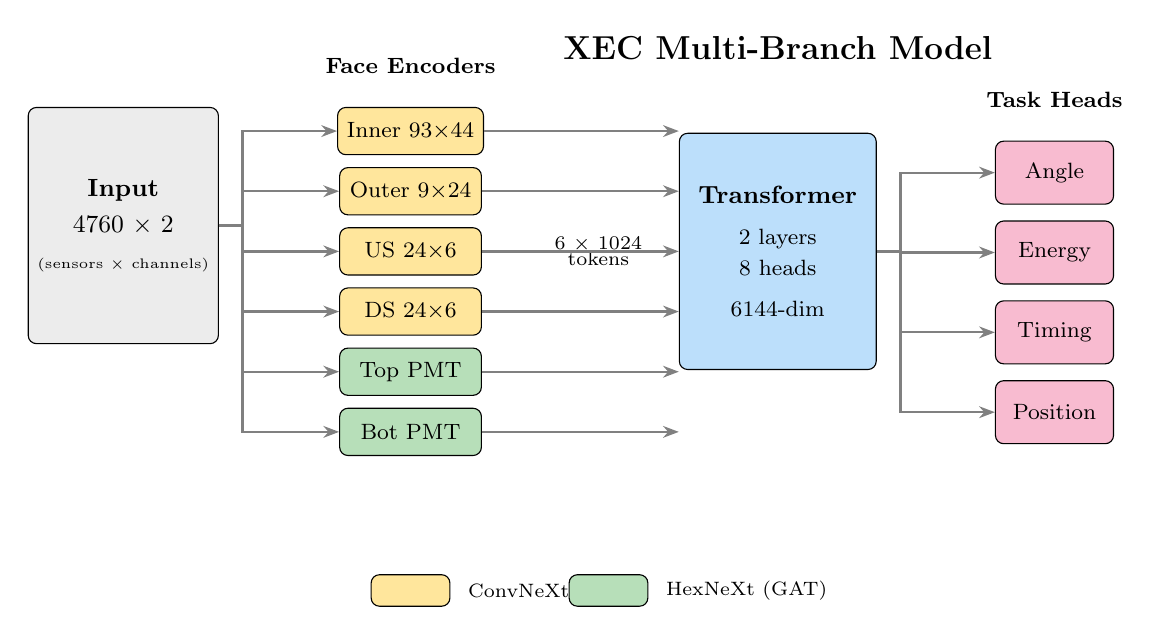
\begin{tikzpicture}[
    node distance=0.6cm and 1.2cm,
    every node/.style={font=\small},
    block/.style={rectangle, draw, rounded corners=3pt, minimum height=0.8cm, align=center},
    input/.style={block, fill=InputColor!20, minimum width=2cm},
    encoder/.style={block, minimum width=1.8cm, minimum height=0.6cm},
    conv/.style={encoder, fill=ConvColor!40},
    hex/.style={encoder, fill=HexColor!40},
    fusion/.style={block, fill=FusionColor!30, minimum width=2.5cm, minimum height=3cm},
    head/.style={block, fill=HeadColor!30, minimum width=1.5cm},
    arrow/.style={-{Stealth[length=2mm]}, thick, gray},
    brace/.style={decorate, decoration={brace, amplitude=5pt, raise=2pt}},
]

% Input
\node[input, minimum height=3cm] (input) {
    \textbf{Input}\\[2pt]
    4760 $\times$ 2\\[2pt]
    \tiny(sensors $\times$ channels)
};

% Face Encoders
\node[conv, right=1.5cm of input, yshift=1.2cm] (inner) {\footnotesize Inner 93$\times$44};
\node[conv, below=0.15cm of inner] (outer) {\footnotesize Outer 9$\times$24};
\node[conv, below=0.15cm of outer] (us) {\footnotesize US 24$\times$6};
\node[conv, below=0.15cm of us] (ds) {\footnotesize DS 24$\times$6};
\node[hex, below=0.15cm of ds] (top) {\footnotesize Top PMT};
\node[hex, below=0.15cm of top] (bot) {\footnotesize Bot PMT};

% Encoder label
\node[above=0.3cm of inner, font=\footnotesize\bfseries] {Face Encoders};

% Token notation
\node[right=0.8cm of us, font=\scriptsize, align=center] (tokens) {
    6 $\times$ 1024\\[-2pt]
    tokens
};

% Transformer
\node[fusion, right=2.5cm of us] (trans) {
    \textbf{Transformer}\\[4pt]
    \footnotesize 2 layers\\
    \footnotesize 8 heads\\[4pt]
    \footnotesize 6144-dim
};

% Task Heads
\node[head, right=1.5cm of trans, yshift=1cm] (angle) {\footnotesize Angle};
\node[head, below=0.2cm of angle] (energy) {\footnotesize Energy};
\node[head, below=0.2cm of energy] (timing) {\footnotesize Timing};
\node[head, below=0.2cm of timing] (pos) {\footnotesize Position};

% Head label
\node[above=0.3cm of angle, font=\footnotesize\bfseries] {Task Heads};

% Arrows from input
\foreach \enc in {inner, outer, us, ds, top, bot} {
    \draw[arrow] (input.east) -- ++(0.3,0) |- (\enc.west);
}

% Arrows to transformer
\foreach \enc in {inner, outer, us, ds, top, bot} {
    \draw[arrow] (\enc.east) -- (\enc.east -| trans.west);
}

% Arrows to heads
\foreach \h in {angle, energy, timing, pos} {
    \draw[arrow] (trans.east) -- ++(0.3,0) |- (\h.west);
}

% Legend
\node[conv, below=1.5cm of bot, minimum width=1cm, minimum height=0.4cm] (leg1) {};
\node[right=0.1cm of leg1, font=\scriptsize] {ConvNeXt V2};
\node[hex, right=1.5cm of leg1, minimum width=1cm, minimum height=0.4cm] (leg2) {};
\node[right=0.1cm of leg2, font=\scriptsize] {HexNeXt (GAT)};

% Title
\node[above=0.8cm of trans, font=\large\bfseries] {XEC Multi-Branch Model};

\end{tikzpicture}
\end{document}
